\documentclass[a4paper]{article}
\usepackage{vntex}
\usepackage{subfig}
%\usepackage[english,vietnam]{babel}
%\usepackage[utf8]{inputenc}
%\usepackage[utf8]{inputenc}
%\usepackage[francais]{babel}
\usepackage{a4wide,amssymb,epsfig,latexsym,multicol,array,hhline,fancyhdr}
\usepackage[left=1in,right=0.79in,top=1 in,bottom=1 in]{geometry}
\usepackage{amsmath}
\usepackage{lastpage}
\usepackage[lined,boxed,commentsnumbered]{algorithm2e}
\usepackage{enumerate}
\usepackage{niceframe}
\usepackage{color}
\usepackage{framed}
\usepackage{fancybox}
\usepackage{wrapfig}
\usepackage{subfig}
%\usepackage{mathptmx}
\pagestyle{empty}
\usepackage{graphics}							% Standard graphics package
\usepackage{array}
\usepackage{longtable}
\usepackage{tabularx, caption}
\usepackage{multirow}
\usepackage{multicol}
\usepackage{rotating}
\usepackage{graphics}
\usepackage{geometry}
\usepackage{setspace}
\usepackage{epsfig}
\usepackage{tikz}
\usepackage{indentfirst}
\usepackage{amsfonts}
\usepackage{amssymb}
\usetikzlibrary{arrows,snakes,backgrounds}
\usepackage{hyperref}
\hypersetup{urlcolor=blue,linkcolor=black,citecolor=black,colorlinks=true} 
%\usepackage{pstcol} 								% PSTricks with the standard color package

%\usepackage{fancyhdr}
\setlength{\headheight}{40pt}
\pagestyle{fancy}
\fancyhead{} % clear all header fields
\fancyhead[L]{
 \begin{tabular}{rl}
    \begin{picture}(25,15)(0,0)
    \put(0,-8){
\includegraphics[width=8mm, height=8mm]{hcmut.jpg}}
    %\put(0,-8){\epsfig{width=10mm,figure=hcmut.eps}}
   \end{picture}&
% 	\includegraphics[width=8mm, height=8mm]{hcmut_0.png} & %
	\begin{tabular}{l}
		\textbf{\bf \ttfamily {\color[named]{blue}Trường Đại Học Bách Khoa Tp.Hồ Chí Minh}}\\
		\textbf{\bf \ttfamily {\color[named]{blue}Khoa Khoa Học và Kỹ Thuật Máy Tính}}
	\end{tabular} 	
 \end{tabular}
}
\fancyhead[R]{
	\begin{tabular}{l}
		\tiny \bf \\
		\tiny \bf 
	\end{tabular}  }
\fancyfoot{} % clear all footer fields
\fancyfoot[L]{\scriptsize \ttfamily Bài tập lớn môn: Hệ thống thông minh - Niên khóa: 2020-2021}
\fancyfoot[R]{\scriptsize \ttfamily Trang {\thepage}/\pageref{LastPage}}
\renewcommand{\headrulewidth}{0.3pt}
\renewcommand{\footrulewidth}{0.3pt}

%%%
\setcounter{secnumdepth}{4}
\setcounter{tocdepth}{3}
\makeatletter


\newcounter {subsubsubsection}[subsubsection]
\renewcommand\thesubsubsubsection{\thesubsubsection .\@alph\c@subsubsubsection}
\newcommand\subsubsubsection{\@startsection{subsubsubsection}{4}{\z@}%
	{-3.25ex\@plus -1ex \@minus -.2ex}%
	{1.5ex \@plus .2ex}%
	{\normalfont\large\bfseries}}
\newcommand*\l@subsubsubsection{\@dottedtocline{3}{10.0em}{4.1em}}
\newcommand*{\subsubsubsectionmark}[1]{}
\makeatother
\everymath{\color{black}}
\sloppy
\captionsetup[figure]{labelfont={small,bf},textfont={small,it},belowskip=-1pt,aboveskip=-9pt}

\captionsetup[table]{labelfont={small,bf},textfont={small,it},belowskip=-1pt,aboveskip=7pt}

\setlength{\floatsep}{5pt plus 2pt minus 2pt}
\setlength{\textfloatsep}{5pt plus 2pt minus 2pt}
\setlength{\intextsep}{10pt plus 2pt minus 2pt}
%\setlength{\parindent}{0pt}

\begin{document}

\begin{titlepage}
\begin{center}
			
			\textbf{ {\Large ĐẠI HỌC QUỐC GIA THÀNH PHỐ HỒ CHÍ MINH \\
					TRƯỜNG ĐẠI HỌC BÁCH KHOA \\ \underline{Khoa Khoa học - Kĩ thuật Máy tính }} \\ 
			}
			
		\end{center}

\vspace{1cm}

\begin{figure}[h!]
			\begin{center}
				
\includegraphics[width=6cm]{hcmut.jpg}
			\end{center}
		\end{figure}

\vspace{1cm}


\begin{center}
			\begin{tabular}{c}

% 		\textbf{{\Large Mini Project}}\\
				\textbf{{\Large	 MÔN: HỆ THỐNG THÔNG MINH }}\\
				
			~~\\
				\hline
				\\
		\multicolumn{1}{c}{\textbf{{\Large ĐỀ TÀI: NHẬN DẠNG CHỮ SỐ VIẾT TAY
		}}}
	
		\\

				\\
		\fontsize{18pt}{18pt}\selectfont	%	\textbf{{LAB 3}}\\
	
				\\
				\hline
			\end{tabular}
		\end{center}

\vspace{3cm}

\begin{table}[h]
			\begin{tabular}{rrl}
				\hspace{4 cm} & GVHD: & PGS.TS. Quản Thành Thơ\\[0.5cm]
				& SV thực hiện: & Tô Duy Hưng  -- 1810198\\
				& & Lê Đức Huy -- 1810166\\
				& & Đỗ Lê Quang Trung -- 1811304\\
			
			\end{tabular}
		\end{table}

\vspace{2.4cm}
		\begin{center}
			\bf{ {\large TP. HỒ CHÍ MINH, THÁNG 04/2021}}\\
		\end{center}
\end{titlepage}

%\thispagestyle{empty}

\newpage
\tableofcontents
\newpage

%%%%%%%%%%%%%%%%%%%%%%%%%%%%%%%%%

% \chapter{Logistic Regression}
%%%%%%% Begin subsection %%%%%%%

%%%%%%%% lời giới thiệu

\section{Giới thiệu mạng nơ-ron tích chập (Convolutional Neural Network)}

\subsection{Lịch sử  mạng nơ-ron tích chập}

Mạng Nơ-ron tích chập (Convolutional Neural Network, còn được viết tắt là
CNN hay ConvNet) là một trong những nền tảng quan trọng của chuyên ngành Thị
giác máy tính (Computer Vision) nói riêng, hay của ngành Học sâu (Deep learrning)
nói chung. CNN được chuyên dùng cho các bài toán liên quan đến hình ảnh như
phân loại, phân tích hình ảnh (image classification) hay nhận diện khuôn mặt (facial
recognition).

Không nhiều người biết rằng thiết kế của mạng nơ-ron tích chập tuân theo quá trình xử lý thị giác trong các sinh vật sống. Lấy cảm hứng từ nghiên cứu của Hubel và Wiesel trong những năm 1950 và 1960 về các tế bào thần kinh phản ứng riêng với các kích thích thị giác ở mèo và khỉ, một khái niệm tên là "Neocognitron" đã được Kunihiko Fukushima giới thiệu vào năm 1980. Đây được xem là mạng nơ-ron tích chập đầu tiên xuất hiện trên thế giới. "Neocognitron" giới thiệu hai loại tầng cơ bản: một là tầng S-cells được sử dụng để trích xuất các thuộc tính cục bộ (local feature) của hình ảnh, tương đương với simple cell (dùng để xử lý các đường thẳng cơ bản); hai là C-cells được dùng để giảm thiểu các sai sót khi kết hợp nhiều thuộc tính cục bộ với nhau (tương đương với complex cell). Các thuộc tính cục bộ được tích hợp dần và phân loại ở các tầng sâu hơn. Từ đó máy tính sẽ nhận dạng được các đặc điểm khác nhau của hình ảnh trong quá trình học và có thể phân loại được hình ảnh dựa trên các bộ lọc (filter) khác nhau.  

Từ đó, mạng nơ-ron tích chập ngày càng được phát triển và cho đến thời điểm hiện tại, khi nhắc về khái niệm này, nhiều người trong chúng ta sẽ nghĩ ngay đến hệ thống nhận dạng chữ viết tay
cho zipcode của nhà nghiên cứu Yann LeCun. Ông ấy cùng các cộng sự đã sử dụng Lan truyền ngược (Backpropagation) để tìm hiểu các hệ số nhân tích chập trực tiếp từ hình ảnh của các số viết tay. Do đó, việc học được thực hiện hoàn toàn tự động, hoạt động tốt hơn so với thiết kế hệ số thủ công và phù hợp với một loạt các vấn đề nhận dạng hình ảnh và các loại hình ảnh. Cách tiếp cận này đã trở thành nền tảng của Thị giác máy tính hiện đại.

Có thể thấy, mặc dù CNN được phát minh vào những năm 1980, nhưng bước đột phá của chúng chỉ thực sự bắt đầu vào những năm 2000 với sự phát triển của ngành công nghiệp Trò chơi điện tử. Các card đồ họa ngày càng được nâng cấp để nâng cao trải nghiệm chơi game cho người dùng, mà cốt lõi chính là việc tăng cường khả năng tính toán của các bộ xử lý đồ họa (GPU- Graphic Processing Units). Thoạt
nghe thì có vẻ CNN không dính dáng tới GPU lắm vì chúng thuộc 2 chuyên ngành khác biệt, nhưng thực tế chúng đều hoạt động dựa trên các thao tác với ma trận (matrix manipulation). Hình ảnh là một ma trận các điểm ảnh (pixel), còn video thì ghép nối nhiều hình ảnh khác nhau trong một khoảng thời gian nhất định (60 frame
per second chẳng hạn) để tạo nên những chuyển động. Do tính chất này, GPU được cải thiện sao cho việc tính toán các ma trận pixel được diễn ra nhanh nhất có thể, điều này vô tình khiến các mạng nơ-ron nhân tạo được hưởng lợi rất nhiều. Theo đánh giá của các nhà khoa học thì hiện nay việc triển khai các mô hình mạng CNN trên GPU đạt tốc độ nhanh hơn 20 lần so với việc triển khai tương đương trên CPU.


\subsection{Đặc tính cơ bản của mạng nơ-ron tích chập}
Vậy tại sao mạng nơ-ron tích chập lại được sử dụng phổ biến cho các bài toán phân
tích hình ảnh? Câu trả lời đến từ một bản chất tự nhiên của CNN, đó là khả năng rút trích thuộc tính ẩn (latent feature extraction) cực kỳ tốt. 

Trái ngược với mô hình mạng nơ-ron truyền thẳng  (Feedforward Neural Network) - mô hình mà ở đó các tầng kết nối đầy đủ trực tiếp với nhau thông qua một trọng số w (weighted vector) - thì ở CNN, các tầng liên kết được với nhau thông qua cơ chế tích chập (convolution). Tầng tiếp theo là kết quả tích chập từ tầng trước đó, nhờ vậy mà ta có được các kết nối cục bộ. Nghĩa là mỗi nơ-ron ở tầng tiếp theo sinh ra từ bộ lọc (filter) áp đặt lên một vùng ảnh cục bộ của nơ-ron tầng trước đó. Mỗi tầng như vậy được áp đặt các bộ lọc khác nhau, thông thường có vài trăm đến vài nghìn bộ như vậy. Một số tầng khác như tổng hợp (pooling) hay lấy mẫu con (subsampling)
dùng để chắt lọc lại các thông tin hữu ích hơn (loại bỏ các thông tin nhiễu).

Trong suốt quá trình huấn luyện, CNN sẽ tự động học được các thông số cho các bộ lọc. Ví dụ trong tác vụ phân lớp ảnh, CNN sẽ cố gắng tìm ra thông số tối ưu cho các bộ lọc tương ứng theo thứ tự \textbf{raw pixel $\rightarrow$ cạnh (edges) $\rightarrow$ hình dạng (shapes) $\rightarrow$ khuôn mặt (facial) $\rightarrow$ các đặc trưng mức cao (high-level features)}. Còn lại tầng cuối cùng thì được dùng để phân lớp ảnh. 

Mạng nơ-ron tích chập có tính bất biến và tính kết hợp cục bộ (Location Invariance and Compositionality). Với cùng một đối tượng, nếu đối tượng này được chiếu theo các gốc độ khác nhau như phép dịch chuyển (translation), phép quay (rotation) và phép co giãn (scaling) thì độ chính xác của thuật toán sẽ bị ảnh hưởng đáng kể. Tầng tổng hợp (pooling layer) sẽ cho ta tính bất biến đối với các phép biến hình đã nêu trên. Tính kết hợp cục bộ cho ta các cấp độ biểu diễn thông tin từ mức độ thấp đến mức độ cao và trừu tượng hơn thông qua việc tích chập từ các bộ lọc. Đó là lý do tại sao CNN cho ra mô hình với độ chính xác rất cao. Cách tiếp cận này cũng giống như cách con người nhận biết các vật thể trong tự nhiên. Lấy một ví dụ cụ thể về việc so sánh một con chó và một con mèo, thì cả con người và CNN đều có thể biết cách phân biệt nhờ vào các đặc trưng từ mức độ thấp (có 4 chân, có đuôi) đến mức độ cao (dáng đi, hình thể, màu lông).


\section{Cách thức hoạt động của mạng nơ-ron tích chập}

\subsection{Phép tích chập (Convolution)}

Đúng như cái tên của CNN, phép tính tích chập (convolution) chính là đặc trưng
mạng nơ-ron này. Để có thể dễ dàng nắm bắt được ý tưởng của phép tích chập, ta
hãy cùng phân tích ví dụ sau đây.

Xét một hình ảnh được biểu diễn dưới dạng ma trận X kích thước 5x5 với các phần tử là
chữ số 0 hoặc 1 và một cửa sổ tích chập W (cửa
sổ trượt) là ma trận 3 × 3 như hình \ref{fig:convolution}. 

\begin{figure}[!h]
    \centering
    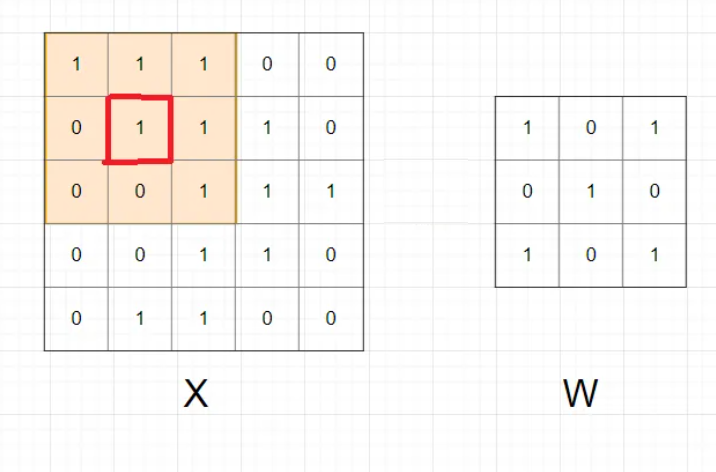
\includegraphics[width=0.8\textwidth]{image/convolution.png}
    \caption{Hình ảnh mô tả ma trận hình ảnh (X) và cửa sổ tích chập (W)}
    \label{fig:convolution}
\end{figure}

Ta có cách tính một phần tử của ma
trận kết quả từ phép tích chập như sau: 

\begin{itemize}
    \item Nhân tích chập cửa sổ trượt W với ma trận con 3x3 tại vị trí đầu tiên của ma
trận hình ảnh X - ma trận được tô màu cam trong Hình \ref{fig:convolution}. Phép nhân tích chập được thực hiện bằng cách nhân từng phần
tử của ma trận hình ảnh con với phần tử tại ví trí tương ứng của cửa sổ trượt
sau đó cộng các kết quả lại. Kết quả cuối cùng chính là giá trị của phần tử
đầu tiên trong ma trận kết quả Y. 

Ví dụ nếu gọi $x_{i,j}$, $y_{i,j}$ và $w_i,j$ lần lượt là các phần tử tại vị trí hàng i cột j của các ma trận X, Y, W thì $y_{1,1} = x_{1,1}*w_{1,1}+x_{1,2}*w_{1,2}+x_{1,3}*w_{1,3}+x_{2,1}*w_{2,1}+x_{2,2}*w_{2,2}+x_{2,3}*w_{2,3}+x_{3,1}*w_{3,1}+x_{3,2}*w_{3,2}+x_{3,3}*w_{3,3} = 1 * 1 + 1 * 0 + 1 * 1 + 0 * 0 + 1 * 1 + 1 * 0 + 0 * 1 + 0 * 0 + 1 * 1 = 4$

\item Tiếp đó, trượt cửa sổ tích chập sang phải của ma trận hình ảnh stride đơn vị cột (khái niệm về stride sẽ được trình bày sau ở mục 2.2, trong ví dụ này ta xét trường hợp đơn giản nhất là stride bằng 1) và tiếp tục nhân tích chập để tìm được phần tử thứ 2 trong ma trận kết quả. Làm liên tục cho đến khi không thể trượt sang phải thêm được nữa. ta có được các phần tử của hàng đầu tiên trong ma trận kết quả tích chập. Kết quả minh họa ở Hình \ref{fig:FR1} và Hình \ref{fig:FR2}.

\begin{figure}[!h]
    \centering
    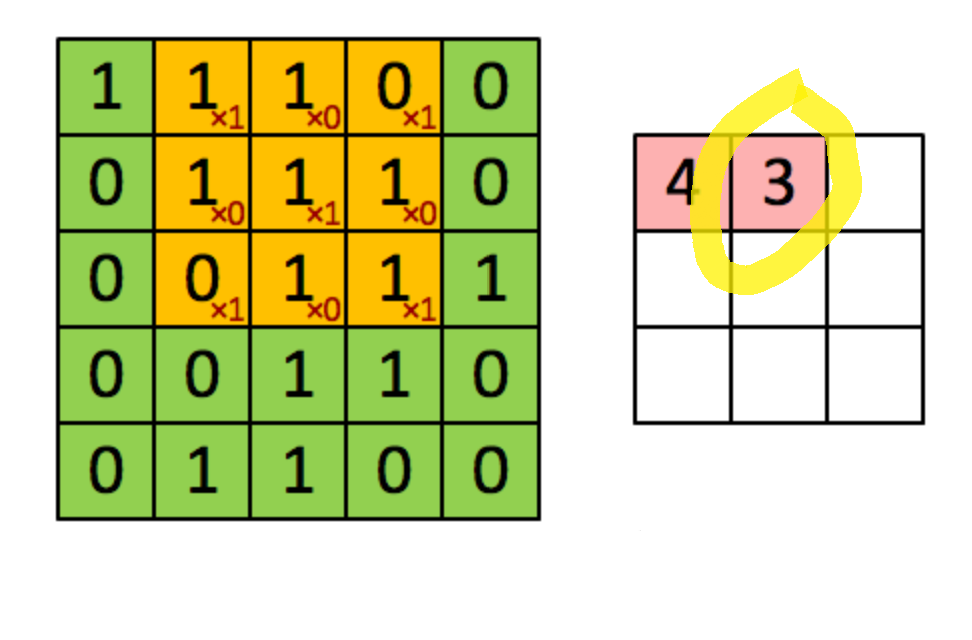
\includegraphics[width=0.4\textwidth]{image/first_row_1.png}
    \caption{Cách tính phần tử hàng 1 cột 2 của Y}
    \label{fig:FR1}
\end{figure}

\begin{figure}[!h]
    \centering
    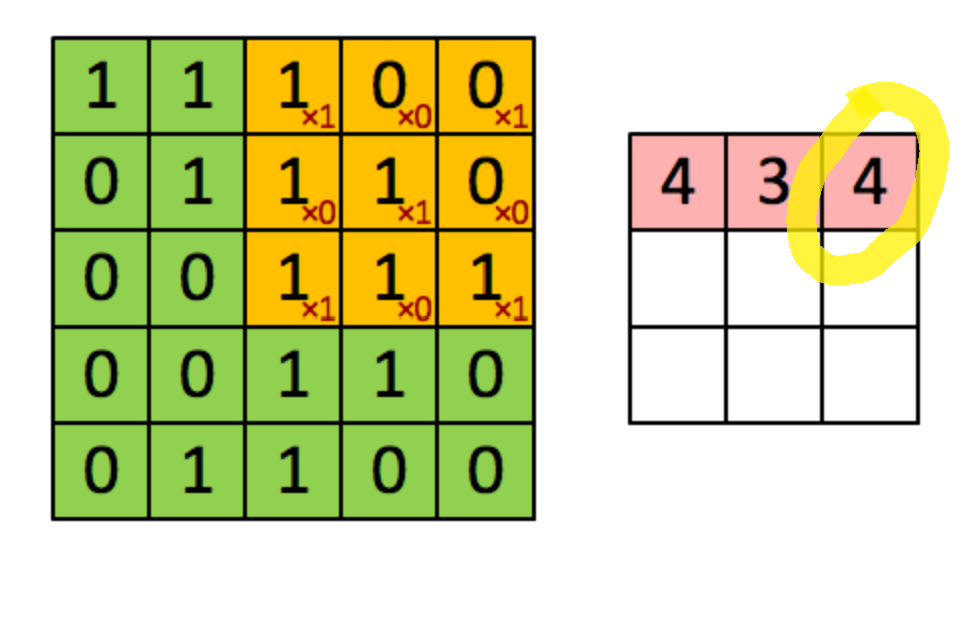
\includegraphics[width=0.4\textwidth]{image/first_row_2.png}
    \caption{Cách tính phần tử hàng 1 cột 3 của Y}
    \label{fig:FR2}
\end{figure}

\item Để tính tiếp các hàng tiếp theo cho ma trận kết quả, ta dời cửa sổ trượt về vị trí đầu tiên - ma trận được tô màu cam trong Hình \ref{fig:convolution} - và trượt cửa sổ xuống stride đơn vị hàng. Tiếp tục lặp lại quá trình nhân tích chập và trượt cửa sổ. Ma trận kết quả sau khi hoàn thành quá trình tích chập sẽ có kích thước 3x3 như hình \ref{fig:conv_result}.

\begin{figure}[!h]
    \centering
    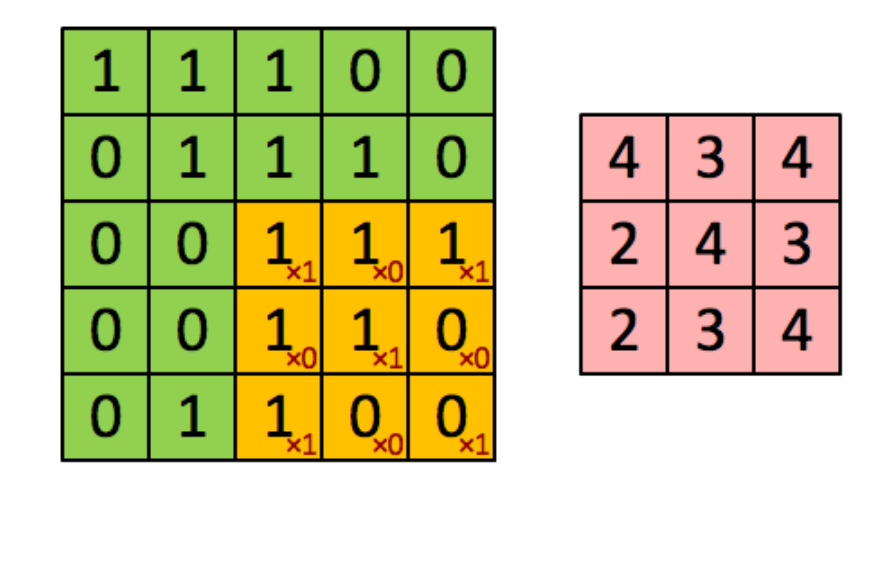
\includegraphics[width=0.4\textwidth]{image/conv_result.png}
    \caption{Hình ảnh mô tả ma trận kết quả Y đầy đủ}
    \label{fig:conv_result}
\end{figure}

Tổng quát hóa ta rút ra công thức sau

$y_{ij}  = \sum_{k=i}^{k+m-1}\sum_{l=j}^{l+m-1}(x_{k,l}*w_{k-i+1,l-j+1})$

Khi đó, kích thước của ma trận Y là (m-k+1) * (n-k+1) với m * n là kích thước của ma trận ảnh đầu vào X. Áp dụng ngay cho ví dụ trên, ta có thể tính được kích thước của ma trận Y là (5 - 3 + 1 ) * (5 - 3 + 1 ) = 3 * 3 mà không cần phải thực hiện chi tiết từng bước tích chập.

\end{itemize}

Như vậy, ta đã có thể nắm được quá trình nhân tích chập diễn ra như thế nào. Để thực hành làm quen với phép tích chập, hãy thử tiếp tục nhân tích chập ma trận hình ảnh ban đầu cho các cửa sổ trượt đặc biệt trong Hình \ref{fig:filter}.

\begin{figure}[!h]
    \centering
    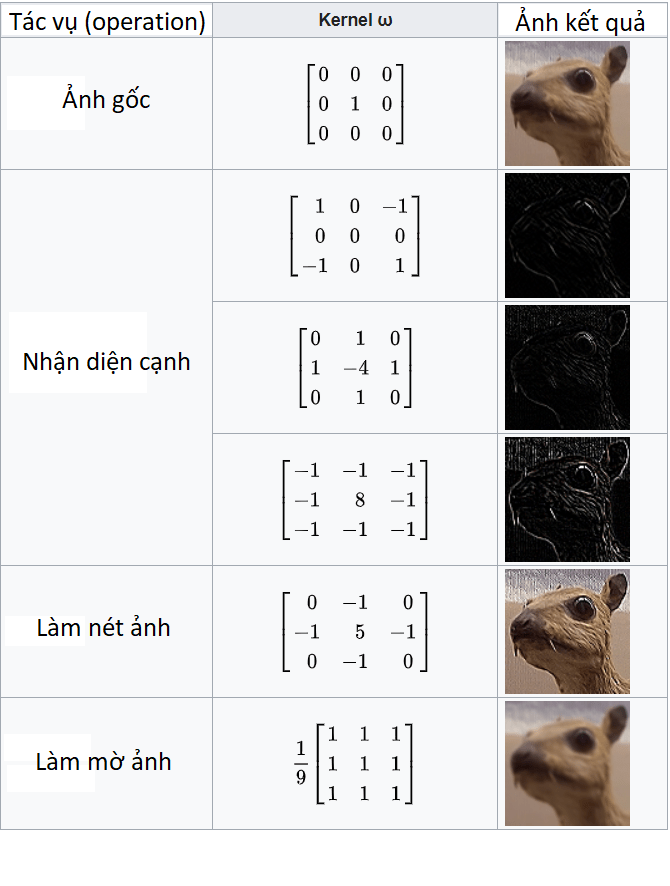
\includegraphics[width=0.5\textwidth]{image/filter.png}
    \caption{Một số bộ lọc đặc biệt}
    \label{fig:filter}
\end{figure}

Những ma trận từ các cửa sổ trượt trên còn được gọi là bộ lọc (filter) bởi vì chúng hoạt động như các bộ lọc trong kỹ thuật xử lý ảnh, có thể được thiết lập để phát hiện các cạnh trong hình ảnh hay làm mờ hình ảnh,... Chính vì vậy, để mạng nơ-ron hoạt động hiệu quả hơn, ta có thể thêm vào nhiều tầng phía  sau tầng đầu vào, mỗi tầng có thể được áp dụng các bộ lọc khác nhau. Nhờ đó, nó có thể trích xuất được nhiều đặc tính quan trọng từ các hình ảnh đầu vào. 

\subsection{Stride}

Trong thực tế, lớp tích chập có nhiều thiết lập khác nhau cung cấp các khả năng để giảm số lượng các tham số, đồng thời làm giảm các tác dụng phụ, một trong số đó là \textit{stride}. Trong các ví dụ được đề cập ở trên, ta giả sử ma trận tích chập trượt lần lượt trên hình ảnh đầu vào, mỗi lần di chuyển 1 đơn vị. Ta có thể thay đổi độ dời của ma trận tích chập mỗi lần di chuyển bằng cách thay đổi \textit{stride}. Ta có thể thấy trong Hình \ref{fig:stride}, với ma trận đầu vào có kích thước 7x7, nếu ta di chuyển ma trận tích hợp 1 đơn vị mỗi lần cho đến hết thì ma trận kết quả sẽ có kích thước 5x5. Nếu ta thay đổi \textit{stride=2}, tức là di chuyển ma trận tích hợp 2 đơn vị mỗi lần thì ma trận kết quả sẽ chỉ có kích thước 3x3.\par

\begin{figure}
    \centering
    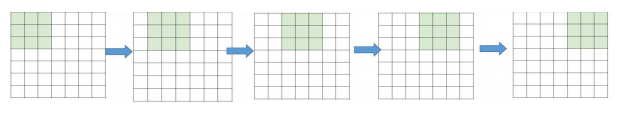
\includegraphics[width=\linewidth]{image/stride.png}
	\caption{Sử dụng stride=1 với ma trận tích chập}
	\label{fig:stride}
\end{figure}

\vspace{0.35cm}

Tổng quát hóa, với ma trận đầu vào có kích thước n * n, ma trận tích hợp có kích thước f * f và giá trị \textit{stride} là s thì ma trận kết quả O sẽ có kích thước là:

\begin{equation*}
( \lfloor \frac{n-f}{s} + 1 \rfloor ) * ( \lfloor \frac{n-f}{s} + 1 \rfloor )
\end{equation*}


%     O = \frac{N-F}{S} + 1
% \end{align*}

\subsection{Padding}

Bởi vì sau mỗi lần thực hiện phép tích chập, kích thước ma trận đầu ra Y đều nhỏ kích thước của ma trận đầu vào X (do m - k + 1 < m) nên một trong những hạn chế của ma trận tích chập là có thể làm mất đi thông tin quan trọng tồn tại trên đường viền của hình ảnh. Để khắc phục hạn chế này, một giải pháp đơn giản đã được đề ra là sử dụng kỹ thuật \textit{zero padding}. Kỹ thuật này cho phép thêm vào các số 0 bên ngoài ma trận đầu vào nhằm tạo ra đường viền ảo cho hình ảnh, giúp ngăn chặn việc kích thước đầu ra giảm dần khi tới các lớp sâu hơn trong mạng nơ-ron, cho phép triển khai các mạng học sâu phức tạp với nhiều tầng tích chập.

Hình là một ví dụ mình họa trực quan cho trường hợp padding = 1. Ma trận X trước khi thực hiện phép tích chập đã được thêm 1 viền số 0 bên ngoài, nhờ đó kích thước ma trận Y thu được sau khi tích chập với kernel có giá trị là (7 - 3 + 1) * (7 - 3 + 1) = 5*5, bằng với kích thước ma trận X ban đầu. Tổng quát hóa với padding = p, ta sẽ thêm p vector 0 vào mỗi phía của ma trận. Kết hợp với giả thiết ma trận đầu vào có kích thước n * n, tích chập với kernel kích thước f * f và giá trị stride = s thì ma trận kết quả Y sẽ có kích thước: 

\begin{equation*}
( \lfloor \frac{n-f+2p}{s} + 1 \rfloor ) * ( \lfloor \frac{n-f+2p[}{s} + 1 \rfloor )
\end{equation*}


\subsection{Phép gộp (Pooling)}
Sau khi có được các ma trận kết quả với kích thước 3x3 từ phép tính tích chập. Ta tiếp tục thực hiện phép gộp (pooling) để tiếp tục thu nhỏ ma trận hình ảnh. Có nhiều cách thực hiện phép gộp khác nhau như: lấy giá trị lớn nhất (max pooling), lấy giá trị trung bình (average pooling) hay lấy giá trị tổng (sum pooling). Trong thực tế, max pooling có khả năng khử nhiễu tốt hơn các loại pooling khác, vì vậy ta sẽ sử dụng max pooling để làm ví dụ minh họa cho phép gộp. Xét ma trận kết quả được tính từ cửa sổ tích gộp đầu tiên. Ta thực hiện phép gộp max pooling như sau:

\begin{itemize}
    \item Chia ma trận kết quả ra thành các ma trận con (grid) có kích thước 2 × 2. Lưu ý là do ma trận kết quả có kích thước là 3 × 3 nên các ma trận con nằm ở cuối hàng và cuối cột chỉ có kích thước 1 × 2 hoặc 2 × 1.
    \item Giá trị lớn nhất trong mỗi ma trận con (khoanh vuông màu đen) chính là phần tử của ma trận gộp mới. Lúc này ma trận kết quả sau khi gộp chỉ còn có kích thước 2 × 2, giảm đáng kể so với ma trận 5 × 5 ban đầu.
\end{itemize}

Hình \ref{fig:pooling} mô tả quá trình thực hiện phép gộp này. Và như vậy, ta đã nắm bắt được ý tưởng của phép gộp (pooling) trong mạng nơ-ron tích chập.

\begin{figure}[h]
    \centering
    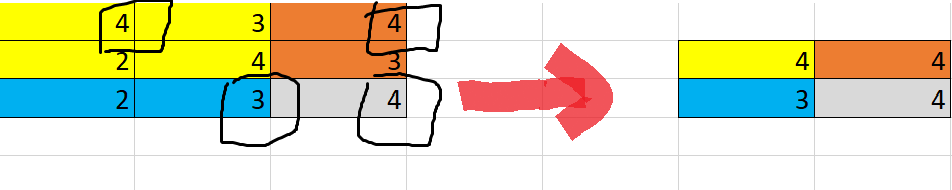
\includegraphics[width=0.8\textwidth]{image/pooling.png}
    \caption{Hình ảnh mô tả ma trận kết quả sau khi thực hiện max pooling}
    \label{fig:pooling}
\end{figure}

\subsection{Ý nghĩa của ma trận kết quả}
Sau khi đã thực hiện phép tích chập (convolution) và phép gộp (pooling), ta có được ma trận kết quả kích thước 2x2 là ma trận sau dấu mũi tên trong Hình \ref{fig:pooling}. Giả sử nếu có thêm 3 cửa sổ trượt nữa, thực hiện tương tự các phép tích chập và phép gộp như đã nêu trên, ta sẽ có 4 ma trận kết quả.

Chọn ra giá trị lớn nhất trong 4 ma trận trên, giả sử là \textit{k}. Khi đó, vì nhận thấy rằng giá trị tối đa có thể có được của mỗi phần tử chỉ có thể là \textit{k} nên ta sẽ thực hiện thêm một biến đổi cho 4 ma trận này bằng cách chuyển các giá trị \textit{k} thành dấu x, các giá trị nhỏ hơn \textit{k} đều được thay bằng 0. Sau phép biến đổi này, ta có được 4 ma trận mới.

Sau khi biến đổi thì các ma trận kết quả sẽ thể hiện được sự phân bố mẫu (pattern) của các cửa sổ trượt nhỏ trên ma trận hình ảnh ban đầu. Đó là lý do vì sao các cửa sổ trượt này được gọi là các bộ lọc (filter). Nhiệm vụ của chúng chính là tìm ra các đặc trưng của hình ảnh. Ở các lớp cao hơn, các bộ lọc đóng các vai trò khác nhau tùy theo yêu cầu của bài tóan như bộ phát hiện cạnh (edge detector), bộ phát hiện nhiễu (noise detector),...

\subsection{Bản đồ thuộc tính (Feature map)}
Nếu ghép 4 ma trận kết quả đã nêu trên lại với nhau, ta được một hình ảnh gọi là bản đồ thuộc tính (feature map), được trích xuất sau quá trình tích chập của mạng CNN. Bản đồ thuộc tính là một đặc trưng nổi bật của mạng nơ-ron tích chập, bởi nó thể hiện được các thuộc tính tiềm ẩn (latent features) của hình ảnh đầu vào.

Cần lưu ý rằng bản đồ thuộc tính được sinh ra dựa trên các bộ lọc đã được định nghĩa trước (hay chính là các cửa sổ tích chập trong ví dụ trên). Do đó, điều quan trọng chính là làm sao định nghĩa được các bộ lọc này một cách phù hợp để áp dụng hiệu quả cho những bài toán cụ thể. Ví dụ như với bài toán nhận diện khuôn mặt người, bộ lọc sẽ là các bộ nhận diện mắt, mũi, miệng. Còn đối với bài toán nhận diện vạch kẻ đường, mạng nơ-ron cần học được các bộ lọc nhận diện đường thẳng,... Vấn đề này sẽ được bàn đến trong phần tiếp theo, khi ta cần sử dụng cơ chế học của mạng nơ-ron nhân tạo thông thường để có thể học được bộ lọc.

\section{Lớp phi tuyến tính}

\vspace{0.35cm}

Lớp tiếp theo sau lớp tích chập mà ta sẽ giới thiệu là lớp phi tuyến tính. Lớp phi tuyến tính có thể được sử dụng để điều chỉnh hoặc cắt bỏ các giá trị trong ma trận đầu ra. Lớp này được áp dụng để bão hòa hay giới hạn các giá trị được tạo ra trong ma trận đầu ra. \par

\vspace{0.35cm}

Trong suốt nhiều năm, các hàm phi tuyến tính được sử dụng nhiều nhất là sigmoid và tanh. Tuy nhiên, hiện tại hàm ReLU (Rectified Linear Unit) được sử dụng phổ biến hơn bởi những lý do sau:

\begin{itemize}
    \item ReLU có định nghĩa đơn giản về cả hàm số lẫn đạo hàm.
    \begin{align*}
        ReLU(x) &= max(0, x)\\
        \frac{d}{dx} ReLU(x) &= 
        \begin{cases} 
            1, & \mbox{nếu } x > 0 \\
            0, & \mbox{nếu } x \leq 0
        \end{cases}
    \end{align*}
    \item Các hàm bão hòa như sigmoid gây ra các vấn đề trong việc truyền ngược. Khi mạng thần kinh được thiết kế sâu hơn, các tín hiệu độ dốc sẽ bị "biến mất", không có ý nghĩa trong quá trình huấn luyện mạng thần kinh. Điều này xảy ra do giá trị độ dốc của các hàm đó rất gần bằng 0 hầu như ở khắp mọi nơi trừ vùng gần giá trị trung bình của hàm. Tuy nhiên, ReLU có một độ dốc không đổi cho đầu vào dương và băng 1. 
    \item ReLU tạo ra các thể diện thưa hơn, bởi vì các giá trị âm đều được chuyển hoàn toàn về 0. Ngược lại, các hàm sigmoid và tanh luôn có kết quả khác 0 về độ dốc, có thể gây bất lợi cho việc huấn luyện mạng thần kinh.
\end{itemize}

\begin{figure}
    \centering
    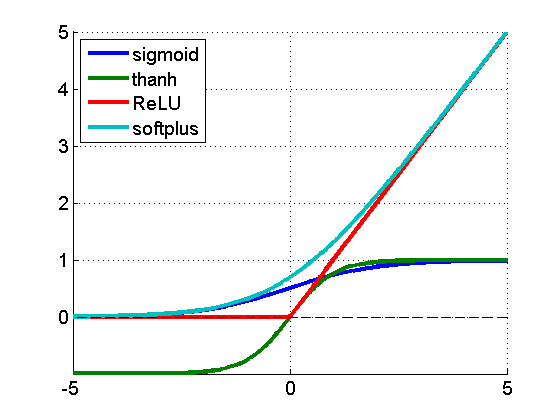
\includegraphics[width=0.6\linewidth]{image/common_nonlinear.png}
	\caption{Các hàm phi tuyến tính phổ biến}
	\label{fig:common_nonlinear}
\end{figure}

\section{Lớp tổng hợp}

\vspace{0.35cm}

Lớp tổng hợp thường được sử dụng giữa các lớp tích chập để đơn giản hóa thông tin đầu vào nhằm làm giảm số lượng neuron ở các lớp tiếp theo trong khi vẫn giữ lại được các đặc tính quan trọng của dữ liệu đầu vào. Điều này giúp làm giảm độ phức tạp và khối lượng tính toán của mạng thần kinh đồng thời vẫn bảo toàn được hiệu suất tính toán và độ chính xác của nó. Trong lĩnh vực xử lý ảnh, việc này tương tự vói giảm độ phân giải của hình ảnh. \par

\vspace{0.35cm}

Các phương pháp tổng hợp được dùng phổ biến hiện nay là tổng hợp trung bình (average pooling) và tổng hợp cực đại (max pooling). Phương pháp tổng hợp cực đại chia hình ảnh ban đầu thành nhiều vùng nhỏ hơn có cùng kích thước và chọn giá trị lớn nhất trong vùng đó làm giá trị đầu ra của 1 neuron trong lớp tiếp theo. Các kích thước vùng thường được dùng để tổng hợp là 2x2 và 4x4. Ta có thể thấy trong Hình \ref{fig:pooling}, khi sử dụng lớp tổng hợp cực đại với kích thước vùng là 2x2, nó sẽ chọn giá trị cực đại trong mỗi vùng (các vùng xanh vàng, cam, xám, xanh dương) và tổng hợp thành ma trận kết quả, ma trận kết quả đã giảm kích thước đi so với ma trận đầu vào. \par



Việc sử dụng các lớp tổng hợp sẽ làm thay đổi vị trí tương đối của các điểm ảnh trong hình ảnh, do đó sẽ không bảo toàn được thông tin ban đầu. Vì vậy, các lớp tổng hợp chỉ nên được sử dụng khi cần trích xuất và bảo toàn các thông tin quan trọng của hình ảnh. Ngoài ra, ta có thể sử dụng các lớp tổng hợp với \textit{stride} khác nhau để tăng độ hiệu quả cho việc trích xuất các đặc tính của dữ liệu đầu vào. 

\section{Lớp kết nối đầy đủ}

\vspace{0.35cm}

Lớp kết nối đầy đủ được xây dựng tương tự như cách sắp xếp các neuron trên một lớp trong các mạng thần kinh nhân tạo cố điển. Trong đó, mỗi neuron ở lớp sau được kết nối tới tất cả các neuron ở lớp trước như trong Hình \ref{fig:fully_connect}. Đây là những lớp rất quan trọng đối với quá trình huấn luyện mạng thần kinh tích chập, giúp mạng thần kinh "học hỏi" được các đặc tính quan trọng của hình ảnh và đưa ra các kết quả dự đoán chính xác nhất. \par

\begin{figure}
    \centering
    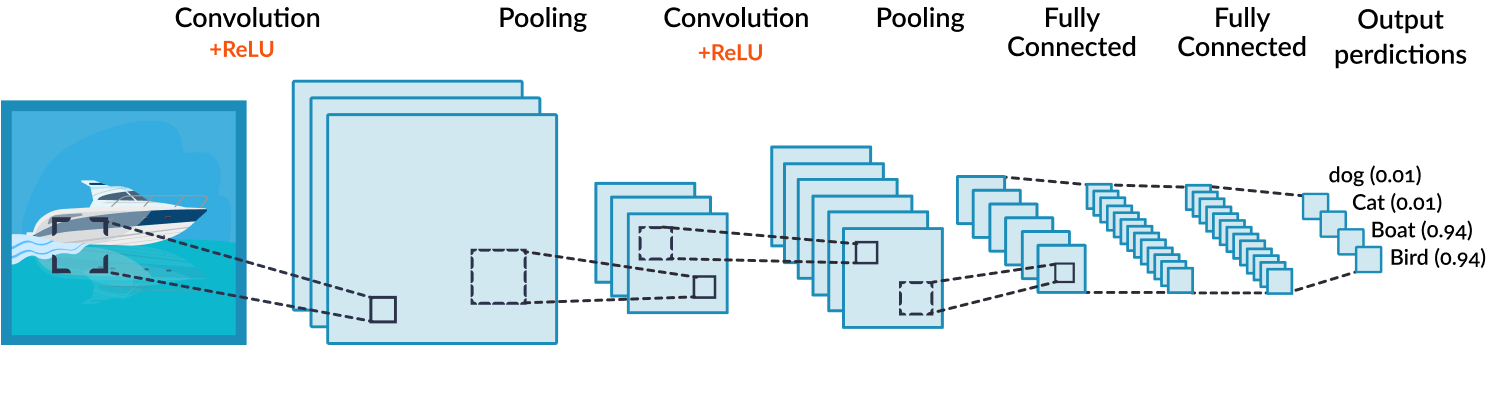
\includegraphics[width=\linewidth]{image/convolution_network.png}
	\caption{Lớp kết nối đầy đủ}
	\label{fig:fully_connect}
\end{figure}

Hạn chế chính của lớp kết nối đầy đủ là nó chứa nhiều tham số và yêu cầu nhiều thao tác tính toán phức tạp trong quá trình huấn luyện mạng thần kinh. Chúng ta có thể loại bỏ một phần các kết nối nhằm tăng tốc độ huấn luyện mà vẫn bảo toàn được hiệu suất và độ chính xác của mạng thần kinh bằng kỹ thuật loại bỏ (dropout). 


\section{Mạng nơ-ron tích chập dưới góc nhìn của một mạng nơ-ron nhân tạo}
Trong một mạng nơ-ron nhân tạo thông thường thì một mạng nơ-ron được cấu thành bởi các nút nơ-ron khác nhau nối tiếp nhau và qua quá trình xử lý thông tin sẽ tạo ra các nút nơ-ron ở tầng tiếp theo. Tương tự như vậy với mạng nơ-ron tích
chập, ví dụ có một hình ảnh được biểu diễn dưới dạng ma trận đầu vào với kích thước 10 × 10 và một cửa sổ tích chập là ma trận 4 × 4 thì quá trình nhân tích chập tại vị trí đầu trên ma trân đầu vào 10 × 10 sẽ tạo ra được một phần tử của ma trận mới và đó cũng tương đương với một nút nơ ron được tạo ra sau khi thực hiện một phép biến đổi. Nút nơ-ron mới sẽ nối với 16 điểm trên ma trận đầu vào.

\begin{figure}
    \centering
    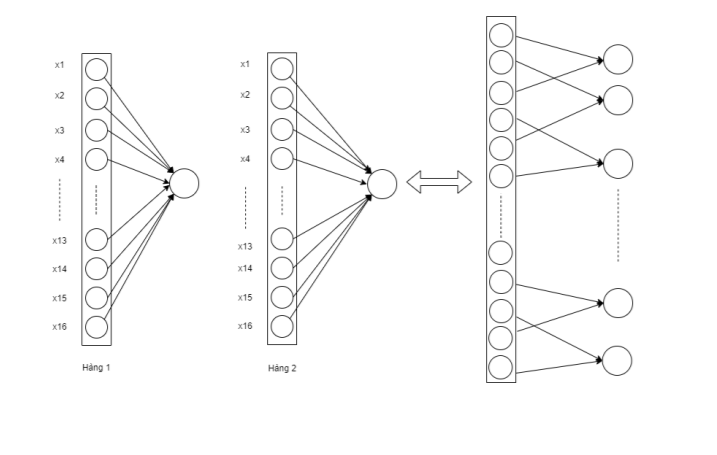
\includegraphics[width=0.9\textwidth]{image/neuronFilter.png}
    \caption{ Hình ảnh mô tả phân tích chập một bộ lọc tạo ra các nơ-ron}
    \label{fig:neuronFilter}
\end{figure}

Hình \ref{fig:neuronFilter} mô tả một ma trận đầu vào cùng với một cửa sổ và khi thực hiện phép tích chập trên một vị trí trên ma trận đầu vào sẽ tạo ra được một nút nơ-ron. Khi cho cửa sổ trượt qua hàng thứ hai sẽ thu được một nơ-ron khá và khi ta cho ma trận
filter này trượt hết trên ma trận đầu vào thì sẽ tạo ra được 49 nút nơ ron khác nhau và mỗi nút nối với một ma trận 16 đơn vị.

Một đặc điểm quan trọng của mạng nơ-ron tích chập là cơ chế chia sẻ trọng số (shared weights). Có nghĩa là các trọng số trên mỗi bộ lọc phải giống nhau và các nơ-ron trong lớp ẩn đầu sẽ phát hiện chính xác điểm tương tự chỉ ở các vị trí khác
nhau trong dữ liệu đầu vào. Việc làm này sẽ làm giảm tối đa số lượng các tham số (parameters), mỗi bản đồ đặc trưng sẽ giúp phát hiện thêm một vài đặc trưng khác. Với một ma trận hình ảnh đầu vào kích thước 10 × 10 như ở trên và 4 bộ lọc có ma trận kích thước 4×4 thì mỗi bản đồ thuộc tính cần 4×4 = 16 trọng số và số nơ-ron được tạo ra ở lớp thứ hai là 49. Như vậy nếu có 4 bản đồ thuộc tính thì có 4 × 16 = 64 tham số. Với một mạng nơ-ron có kết nối đầy đủ thì chúng ta sẽ có 10 × 10 × 49 = 4900 trọng số. Từ kết quả cho thấy sử dụng lớp tích chập sẽ cần số lượng tham số ít hơn nhiều lần so với lớp kết nối đầy đủ nhưng vẫn có thể rút ra các đặc trưng
một cách hiệu quả.

Một khả năng khác của mạng nơ-ron tích chập là số tham số không phụ thuộc vào kích thước của đầu vào. Với những ma trận đầu vào có kích thước khác nhau và thông qua quá trình học theo phương pháp nơ-ron tích chập sẽ rút ra những thuộc tính ẩn mà ta có thể khó nhận thấy. Xét một ví dụ chúng ta có 10 bộ lọc và mỗi một bộ lọc sẽ là một ma trận kích thước 3x3x3 và có một giá trị sai lệch (bias) là 1, chúng ta cần tính xem có bao nhiêu parameter sẽ được tạo ra từ việc sử dụng mạng nơ-ron tích chập? Để giải được bài toàn này thì cần tính số lượng parameters cần dùng mỗi bộ lọc rồi từ đó tính được kết quả.

\begin{itemize}
    \item Số lượng tham số cho mỗi bộ lọc là 3x3x3 = 27
    \item Tổng số tham số cho mỗi bộ lọc là 27 +1 = 28
    \item Tổng số tham số cho 10 bộ lọc là 28 x 10 = 280
\end{itemize}

Như vậy từ ví dụ này thì cho dù dữ liệu đầu vào là bao nhiêu thì số lượng tham số được tạo ra cũng là 280, do đó số tham số có được từ mạng nơ-ron tích chập này không phụ thuộc vào kích thước đầu vào.

\section{Triển khai một mạng CNN}
Một mạng CNN cơ bản bao gồm 3 bộ phận chính: Tầng tích chập (Convolution), tầng tổng hợp (Pooling) và tầng cuối cùng là tầng kết nối đầy đủ (Fully Connected).

Tầng tích chập là tầng quan trọng nhất và cũng là tầng đầu tiên của của mô hình CNN, có chức năng chính là phát hiện các đặc trưng cụ thể của input ban đầu (input ở đây có thể là một bức ảnh cây cối). Tầng này có các bộ phận chính là một ma trận đầu vào, bản đồ thuộc tính (Feature map) và các cửa sổ trượt (Convolution Filter). Tầng này bao gồm nhiều bản đồ thuộc tính đã được trích xuất ra các đặc tính cụ thể, mỗi bản đồ thuộc tính được tạo ra bằng cách quét input ban đầu qua cửa sổ trượt.

Tầng tổng hợp có mục đích làm giảm số lượng thông số mà ta phải tính toán, điều này giúp chúng ta giảm thời gian tính toán. Có 2 phương pháp tổng hợp thường gặp nhất là phép tổng hợp lớn nhất (Max pooling) và phép tổng hợp trung bình
(Average Pooling).

Cuối cùng tầng kết nối đầy đủ sẽ kết hợp các đặc điểm để ra được output của model.
Để dễ hình dung, ta sẽ mô tả mạng quá trình Convolution và Pooling ở ví dụ trước
đó qua hình \ref{fig:convolutionAndPooling} dưới đây.


\begin{figure}
    \centering
    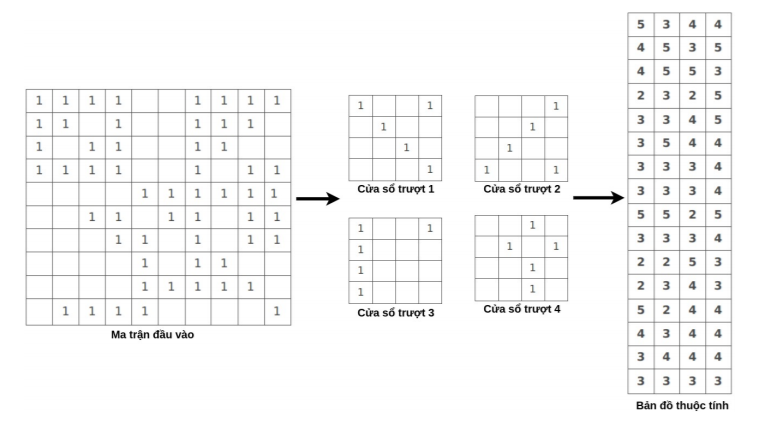
\includegraphics[width=0.8\textwidth]{image/convolutionAndPooling.png}
    \caption{Ví dụ một quá trình Convolution và Pooling}
    \label{fig:convolutionAndPooling}
\end{figure}

Hình \ref{fig:convolutionAndPooling} ở trên biểu diễn ví dụ một ma trận đầu vào có kích thước 10 × 10, 4 cửa sổ trượt, mỗi cửa sổ trượt có kích thước 4x4 và một bản đồ thuộc tính kết quả có kích thước 4 × 16 và một bản đồ thuộc tính kết quả có kích thước 4 × 16. Cách tính toán bao gồm nhân ma trận đầu vào với các cửa sổ trượt, sau đó thực hiện Pooling
để ra được kết quả bản đồ thuộc tính đã được trình bày ở phần trước.

Đây là ví dụ quá trình một ma trận ban đầu được thực hiện Convolution và Pooling để thu được một bản đồ thuộc tính, và quá trình này có thể lặp đi lặp lại nhiều lần nếu cần thiết. Có nghĩa là, bản đồ thuộc tính 4 × 16 ta có được trong ví dụ trên, có thể tiếp tục thực hiện qua các cửa sổ trượt khác, và sẽ thu được một bản đồ thuộc tính khác với cách tính toán tương tự. Quá trình này có thể lặp lại rất nhiều lần, và đến tầng cuối cùng thì ta sẽ học qua tầng Kết nối đầy đủ. Chúng ta cần chú ý rằng quá trình Convolution và Pooling phải được thực hiện ít nhất một lần và 2 tầng này luôn đi kèm với nhau, nhưng luôn cần một tầng kết nối đầy đủ sau cùng, điều này tương đương với việc triển khai một mạng Nơ-ron Network đơn giản cho một bài toán cần học.

Nhưng tại sao tầng cuối phải là fully connected? Ta có thể thấy thực ra việc học
CNN là nó học các trọng số của các cửa sổ trượt, nó cần học và cập nhật lại
các trọng số này. Tương tự như những bài toán trước đó, cần phải có bài toán cho
mạng CNN học. Việc học này sẽ được thực hiện ở tầng fully connected sau cùng,
tương tự như một mạng nơ-ron cơ bản trình bày ở ví dụ trước.


\begin{figure}
    \centering
    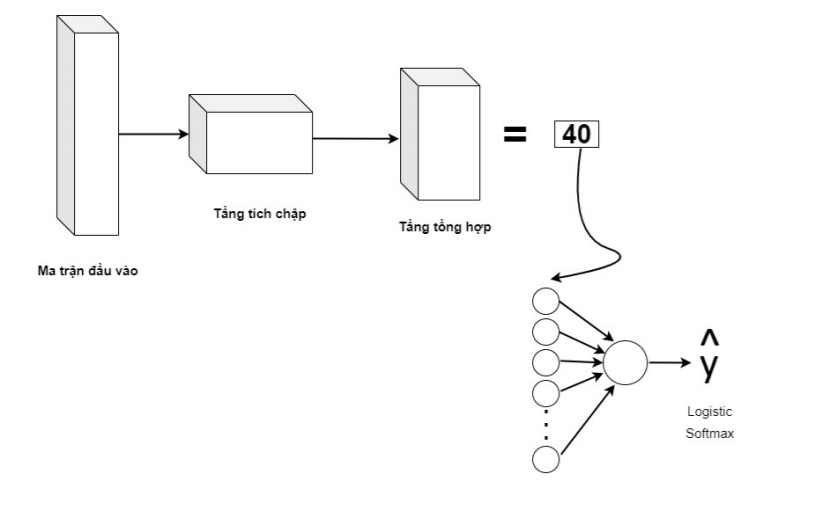
\includegraphics[width=0.8\textwidth]{image/cnnExample.png}
    \caption{Ví dụ một mạng CNN}
    \label{fig:cnnExample}
\end{figure}

Hình \ref{fig:cnnExample} thể hiện ví dụ một mạng CNN, ta có một ma trận đầu vào, một lớp tích
chập và một lớp tổng hợp, ta ví dụ 40 là kết quả tính toán có được sau khi qua lớp
tổng hợp (một vector 40 chiều), và vector 40 chiều này sẽ được đưa vào lớp kết nối
đầy đủ, sử dụng hàm logistic hoặc Softmax tùy theo mục đích, để thu được output
sau cùng.

Và với kiến trúc mạng này, ta có thể ráp nhiều tầng CNN lại với nhau. Ta cũng chú
ý rằng tầng kết nối đầy đủ có thể nhiều hơn 1 tầng để tăng khả năng học của bài
toán cần triển khai, nhưng không nên quá nhiều vì sẽ làm mất đặc trưng của bài toán cần học, vì nếu quá nhiều sẽ dẫn đến việc tăng số lượng thông số đầu vào. Nếu số tầng fully connected quá nhiều thì chỉ riêng thông số của các tầng này cũng đã hơn các tầng trước đó, và điều này làm mất đi một ưu điểm của CNN - giảm số tham số cần học của một mạng học sâu.

Mạng LeNet5 là một trong những mạng CNN lâu đời và nổi tiếng nhất, được Yann LeCUn phát triển vào những năm 1998. Cấu trúc của mạng LeNet5 gồm 2 lớp Convolution và Maxpooling, 2 lớp Fully Connected và output là hàm Softmax. Hình \ref{fig:Lenet5} thể hiện ví dụ một mạng Lenet5.


\begin{figure}[h]
    \centering
    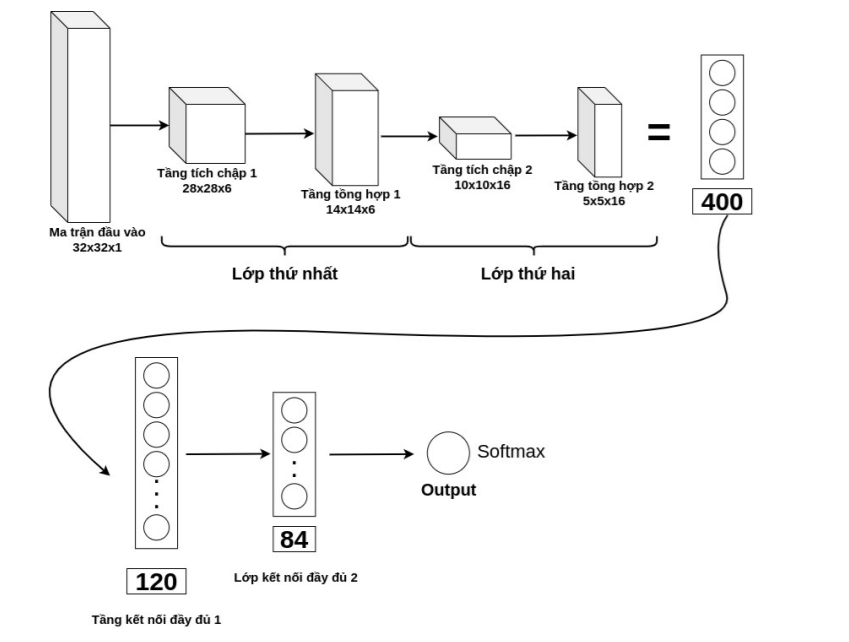
\includegraphics[width=0.8\textwidth]{image/Lenet5.png}
    \caption{Ví dụ một mạng Lenet-5}
    \label{fig:Lenet5}
\end{figure}

Một số thông tin về kiến trúc mạng Lenet5 như sau [18]:
\begin{itemize}
    \item  Đầu vào là một ma trận có kích thước 32 × 32 × 1, nghĩa là một tấm ảnh có chiều dài 32 pixel, chiều rộng ảnh là 32 pixel và số lượng kênh ảnh là 1 (ảnh đen trắng).
    \item  Lớp thứ nhất bao gồm:
    
    – Tầng tích chập thứ 1: là một ma trận 5 × 5 × 3, tốc độ stride là 1, đi qua 6 cửa sổ trượt có kích thước 5 × 5 × 1, và output của nó là 1 ma trận có kích thước 28 × 28 × 6.
    
    – Tầng tổng hợp thứ 1: Kích thước cửa sổ trượt là 1 ma trận 2 × 2, tốc độ stride là 2, số lượng cửa sổ trượt là 16, và output của nó là 1 ma trận có kích thước 14 × 14 × 6.
    \item  Lớp thứ hai bao gồm:
    
    – Tầng tích chập thứ 2: là một ma trận 5 × 5 × 6, tốc độ stride là 1, đi qua 16 cửa sổ trượt và output của nó là 1 ma trận có kích thước 10×10×16.
    
    – Tầng tổng hợp thứ 1: Kích thước cửa sổ trượt là 1 ma trận 2 × 2, tốc độ stride là 2 và output của nó là 1 ma trận có kích thước 5 × 5 × 16.
    \item  Số nút Output của lớp thứ 2 sẽ là 5 × 5 × 16 = 400.
    \item  Số nút Output của tầng kết nối đầy đủ thứ 1 sẽ là 120.
    \item  Số nút Output của tầng kết nối đầy đủ thứ 2 sẽ là 84.
\end{itemize}
Với kiến trúc như thế này, thì việc áp dụng vào từng bài toán cụ thể sẽ được trình bày ở phần sau.


\section{Case study: sử dụng CNN cho bài toán nhận diện chữ số viết tay (Handwriting Recognition)}

Từ những lý do trên, nhóm chúng em quyết định sẽ làm việc với mạng tích chập để giải quyết bài toán phân loại chữ số viết tay từ tập dữ liệu MNIST. MNIST là bộ cơ sở dữ liệu phổ biến về ảnh các chữ số viết tay từ 0 đến 9 bao gồm 2 tập con: tập huấn luyện gồm 60000 ảnh và tập kiểm tra gồm 10000 ảnh. Trong đó mỗi ảnh dữ liệu là một ảnh xám có kích thước 28x28 như Hình \ref{fig:data MNIST} và mục tiêu của bài toán là dự đoán con số viết tay trong bức ảnh đó.

\begin{figure}[h]
    \centering
    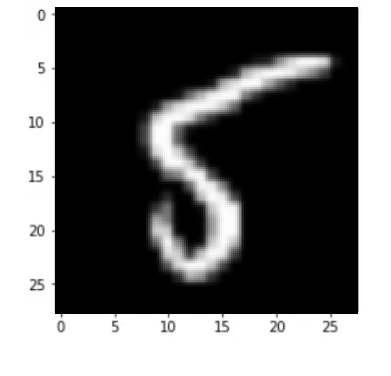
\includegraphics[width=0.3\textwidth]{image/data MNIST.png}
    \caption{Dữ liệu đầu tiên trong tập dữ liệu MNIST}
    \label{fig:data MNIST}
\end{figure}

Nhóm lựa chọn sử dụng thư viện keras hỗ trợ cho quá trình huấn luyện mô hình của mình. Giới thiệu một chút về keras, thì đây là một framework mã nguồn mở về Học sâu được viết bằng ngôn ngữ Python, với các đặc điểm sau:

\begin{itemize}
    \item Việc định nghĩa các tầng (layer), hàm kích hoạt (activation function), hàm mất mát (loss function) thực hiện rất đơn giản.
    \item Chỉ cần định nghĩa mô hình (model) và hàm mất mát, keras sẽ mặc định hỗ trợ người dùng phần Lan truyền ngược (backpropagation).
    \item Việc tính toán được thực hiện tối ưu trên cả CPU và GPU.
\end{itemize}

Vì dữ liệu đầu vào cho mô hình mạng tích chập là 1 tensor 4 chiều (N, W, H, D), cụ thể trong bài toán này là ảnh xám với W = H = 28, D = 1 và N là số lượng ảnh cho mỗi lần huấn luyện, nên trước tiên ta cần reshape lại dữ liệu ảnh có kích thước (N,28,28) thành kích thước (N,28,28,1) để giống kích thước mà keras yêu cầu.

Sau đó, ta xây dựng mô hình cho bài toán theo mạng tích chập như Hình \ref{fig:model MNIST}: từ ảnh đầu vào (input image) đi qua tầng tích chập (convolutional layer), tiếp đến là tầng tổng hợp (pooling layer), và cuối cùng là làm phẳng (flatten) trước khi đưa qua tầng kết nối đầy đủ (fully connected layer) để trả về kết quả đầu ra (output).

\begin{figure}
    \centering
    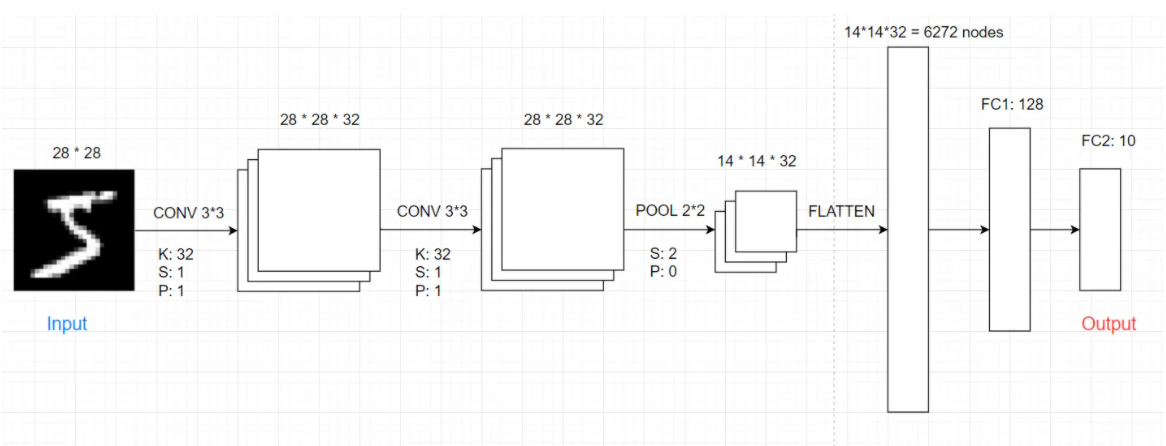
\includegraphics[width=1.0\textwidth]{image/model MNIST.png}
    \caption{Mô hình mạng tích chập để xử lý bài toán}
    \label{fig:model MNIST}
\end{figure}

Chi tiết hơn, khi định nghĩa mô hình bằng cách sử dụng hàm Sequential() - một hàm được hỗ trợ bởi thư viện keras để ta có thể tự sắp xếp các tầng lên nhau trong mô hình mạng tích chập theo ý của mình. Dữ liệu đầu vào lần lượt đi qua các tầng sau
\begin{enumerate}
    \item Tầng tích chập với 32 kernel kích thước 3*3 dùng hàm kích hoạt là hàm ReLU
    \item Tầng tổng hợp
    \item Tầng làm phẳng để chuyển kiểu dữ liệu từ tensor sang vector. Từ tensor có kích thước (14, 14, 32), số nút (node) ta có sau khi làm phẳng là 14 * 14 * 32 = 6272 nút.
    \item Tầng kết nối đầy đủ (FC) với 128 nút và dùng hàm kích hoạt là hàm sigmoid
\end{enumerate}



Vì mỗi ảnh sẽ thuộc 1 lớp (class) từ 0 đến 9 nên ta sẽ có tổng cộng là 10 lớp. Chính vì vậy mà tầng đầu ra sẽ có 10 nút (node) chứa 10 giá trị thực tương ứng với ảnh là số từ 0 đến 9. Gọi $z_{k}$ và $a_{k}$ lần lượt là giá trị thực trong nút và xác suất một tấm ảnh có giá trị là $k$, ta có các công thức tính xác suất cơ bản như sau:

\begin{center}
    $a_{0} = \dfrac{e^{z_{0}}}{e^{z_{0}}+e^{z_{1}}+...+e^{z_{9}}}$ 
    
     $a_{1} = \dfrac{e^{z_{1}}}{e^{z_{0}}+e^{z_{1}}+...+e^{z_{9}}}$ 
     
     ...
     
      $a_{9} = \dfrac{e^{z_{9}}}{e^{z_{0}}+e^{z_{1}}+...+e^{z_{9}}}$ 
\end{center}

Tổng quát hóa thành hàm kích hoạt, ta có công thức: $a_{k} = \dfrac{e^{z_{k}}}{\sum^{10}_{i=1}e^{z_{i}}}$. Đây cũng chính là công thức của hàm kích hoạt softmax.

Khi đã định nghĩa mô hình và hàm kích hoạt, việc cuối cùng ta cần làm đó là định nghĩa hàm mất mát (loss function). Nhưng trước hết, ta phải dùng phương pháp one-hot encoding - một phương pháp phổ biến để mã hóa các dữ liệu rời rạc (categorical data) - nhằm chuyển đổi nhãn của ảnh từ giá trị số nguyên sang vector cùng kích thước với đầu ra của mô hình. Khi đó nhãn của một dữ liệu số i sẽ được mã hóa thành vector v có kích thước 10 * 1 với $v_{i+1}= 1$ và các giá trị còn lại bằng 0. Hình \ref{fig:one hot} là ví dụ minh họa mô tả one-hot vector của dữ liệu số 5.

\begin{figure}
    \centering
    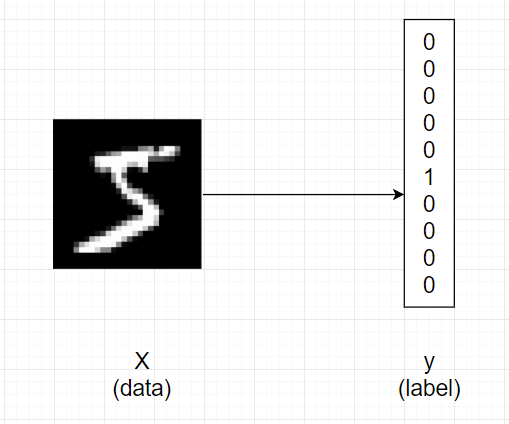
\includegraphics[width=0.6\textwidth]{image/one-hot.png}
    \caption{Hình ảnh mô tả one-hot vector của dữ liệu số 5}
    \label{fig:one hot}
\end{figure}

Giờ ta có cả giá trị thật (label) dạng one-hot encoding và giá trị dự đoán ở tầng đầu ra sau hàm softmax  cùng kích thước 10 * 1. Ta cần định nghĩa hàm mất mát để đánh giá độ tốt của mô hình.

Thực tế, để đánh giá một dữ liệu là số $i$ thì ta càng mong muốn rằng $a_{i}$ càng gần 1 càng tốt còn các giá trị a khác thì ngược lại, càng gần 0 thì càng tốt. Vì như thế cũng đồng nghĩa là mô hình của ta dự đoán đúng được ảnh đầu vào là ảnh số i. Từ ý tưởng này, giả sử $\hat{a}_i$ lần lượt là giá trị dự đoán cho giá trị thực $a_{i}$  ta định nghĩa hàm mất mát như sau:
 
\begin{equation*}
    \centering
    L = - \sum_{i=0}^{9}(a_{i} * log (\hat{a}_{i})
\end{equation*}

Qua đó, ta thấy rằng:

\begin{itemize}
    \item Hàm L giảm dần từ 0 đến 1
    \item Khi model dự đoán \hat{a_i} 
  gần 1, tức giá trị dự đoán gần với giá trị thực $a_i$ thì L nhỏ, xấp xỉ 0
  \item Khi model dự đoán \hat{a_i} 
  gần 0, tức giá trị dự đoán ngược lại giá trị thực $a_{i}$ 
  thì L rất lớn, tiến tới dương vô cùng.
\end{itemize}

Vậy nên có thể kết luận rằng hàm L nhỏ khi giá trị mô hình dự đoán gần với giá trị thực và rất lớn khi mô hình dự đoán sai, hay nói cách khác L càng nhỏ thì model dự đoán càng gần với giá trị chính xác. Khi đó  bài toán tìm mô hình của chúng ta sẽ trở thành bài toán tìm giá trị nhỏ nhất của L.

Hàm mất mát L được định nghĩa như trên trong keras gọi là “categorical\_crossentropy“.


\section{Kết quả}

\subsection{Nhận diện số từ 0 đến 9}

\begin{center}
    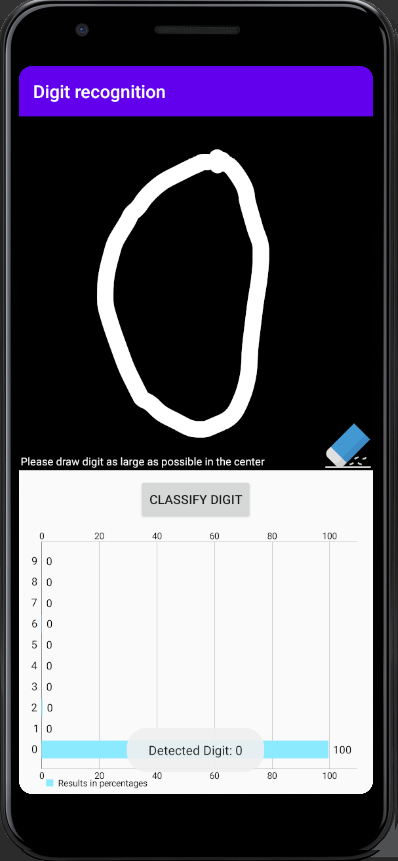
\includegraphics[width=.2\textwidth]{image/num0.png}\hfill
    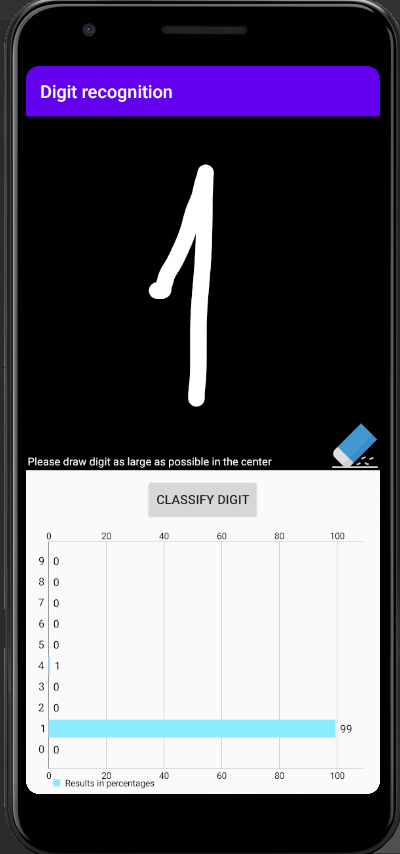
\includegraphics[width=.2\textwidth]{image/num1.png}\hfill
    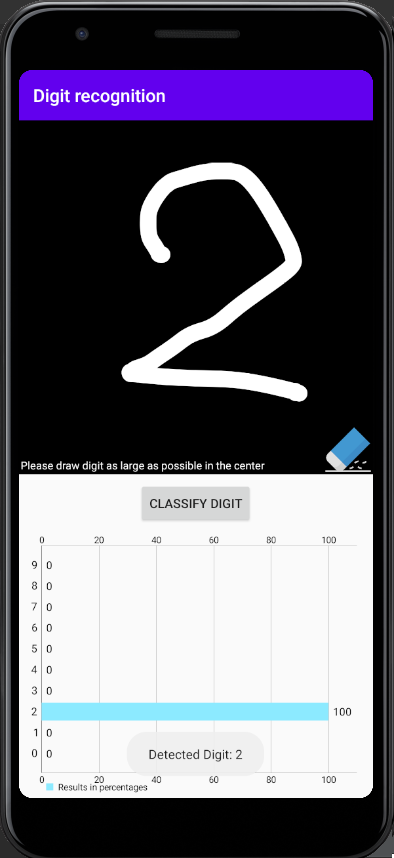
\includegraphics[width=.2\textwidth]{image/num2.png}\hfill
    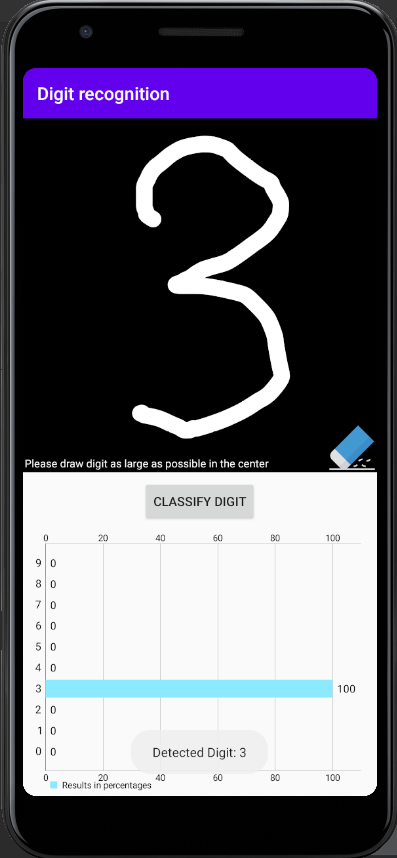
\includegraphics[width=.2\textwidth]{image/num3.png}\hfill
\end{center}

\begin{center}
    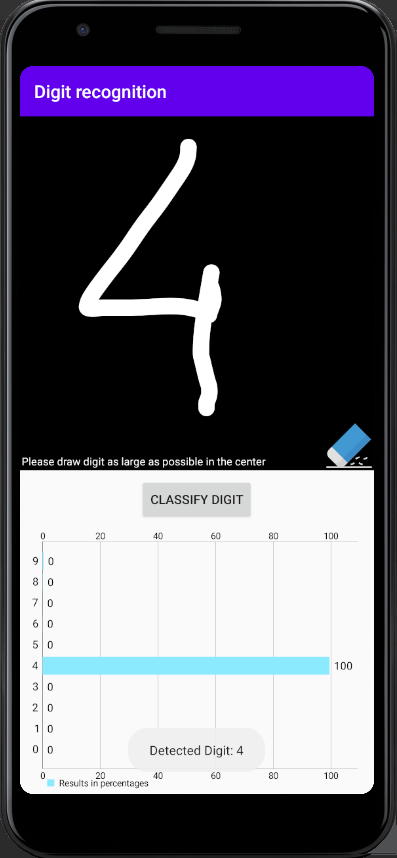
\includegraphics[width=.24\textwidth]{image/num4.png}\hfill
    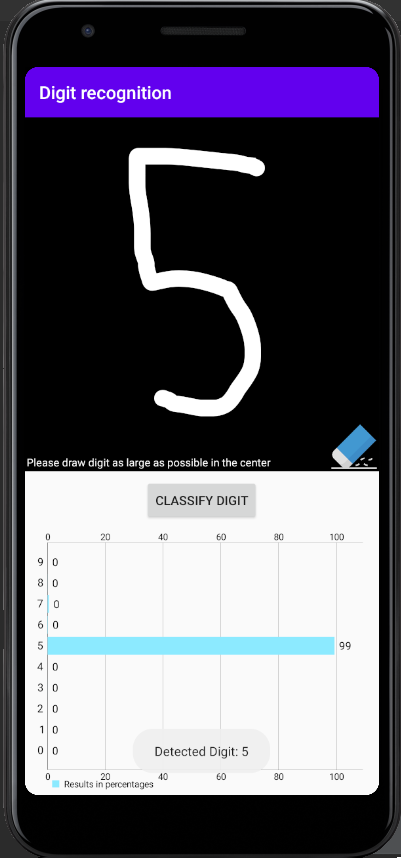
\includegraphics[width=.24\textwidth]{image/num5.png}\hfill
    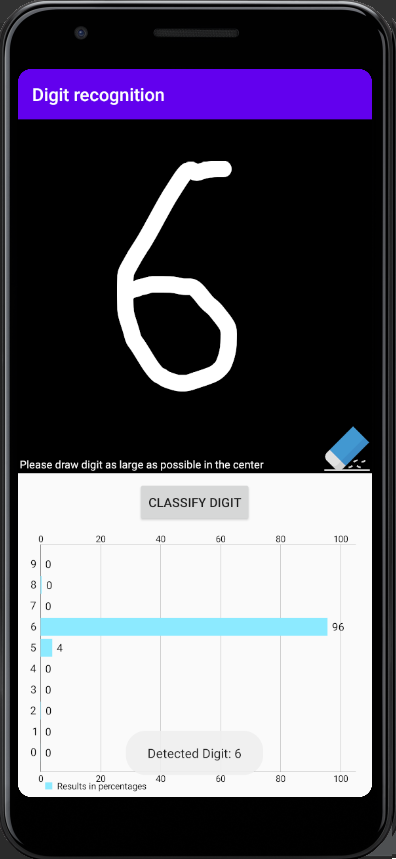
\includegraphics[width=.24\textwidth]{image/num6.png}
\end{center}

\begin{center}
    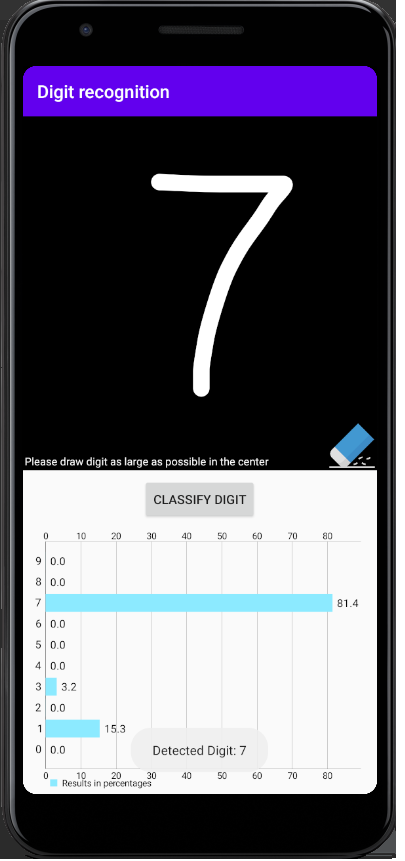
\includegraphics[width=.24\textwidth]{image/num7.png}\hfill
    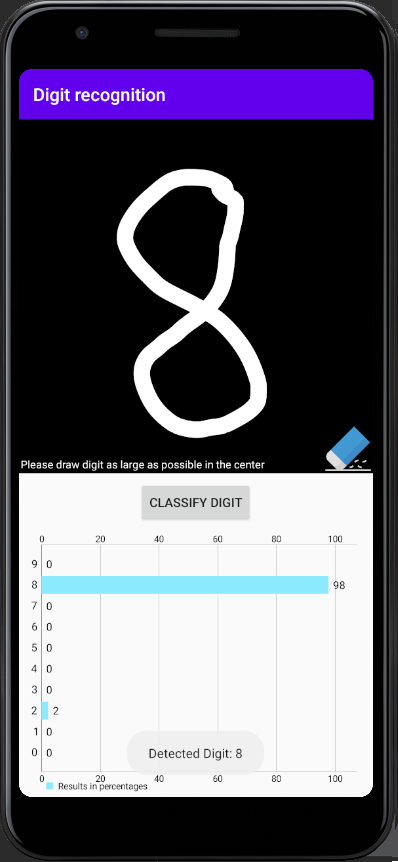
\includegraphics[width=.24\textwidth]{image/num8.png}\hfill
    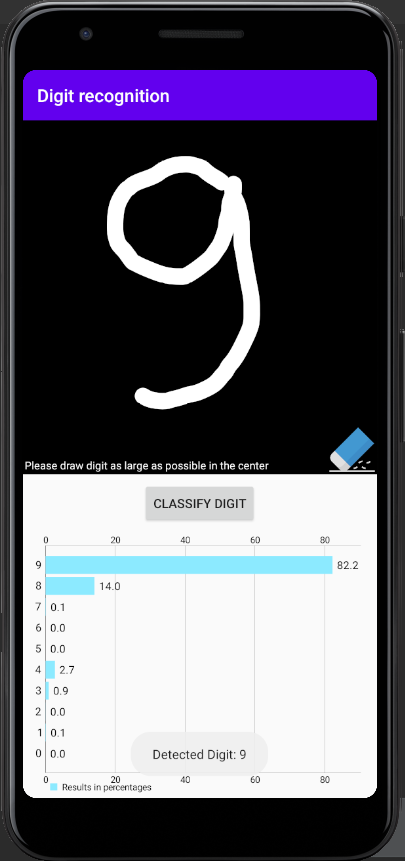
\includegraphics[width=.24\textwidth]{image/num9.png}
\end{center}

\subsection{Những trường hợp viết số không cụ thể}
\begin{center}
    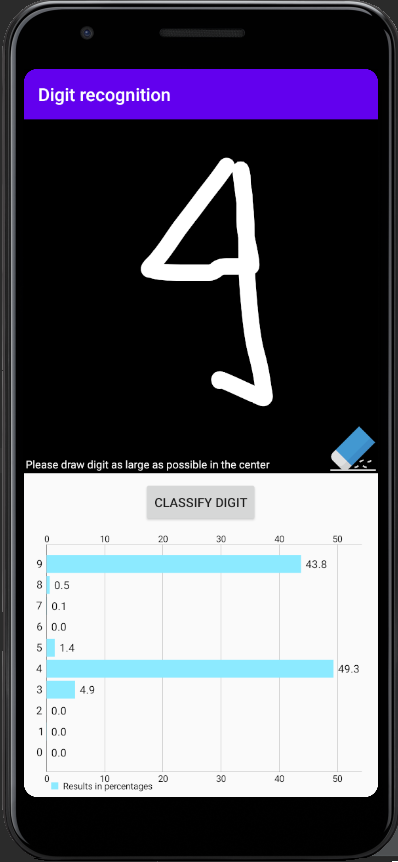
\includegraphics[width=.3\textwidth]{image/special1.png}\hfill
    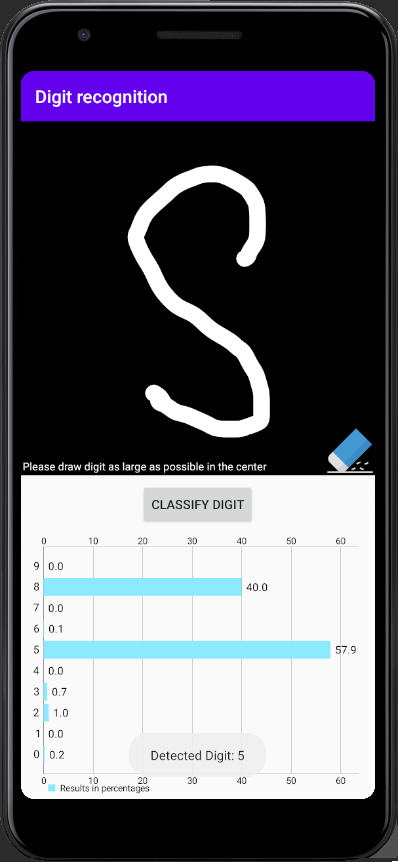
\includegraphics[width=.3\textwidth]{image/special2.png}
\end{center}

Ta thấy, với 2 trường hợp trên, kết quả dự đoán sẽ không chính xác, tỉ lệ dự đoán được phân bố ra các số khác nhau.\\

Tóm lại, độ chính xác của ứng dụng nhận dạng chữ số viết tay sẽ phụ thuộc rất nhiều vào cách người dùng vẽ. Nếu người dùng viết càng rõ ràng, độ chính xác sẽ càng cao. Nếu người dùng viết nguệch ngoạc, không thể hiện số cụ thể, kết quả dự đoán sẽ không chính xác.

\newpage

\textbf{\huge Tài liệu tham khảo} \\\\

[1] O. Abdel-Hamid, L. Deng, and D. Yu, “Exploring convolutional neural network structures and optimization techniques for speech recognition.,” in Interspeech, vol. 11, pp. 73–5, 2013. \\

[2] V. Dumoulin and F. Visin, “A guide to convolution arithmetic for deep learning,” arXivpreprint arXiv:1603.07285, 2016.
\end{document}